\documentclass[a4paper,12pt]{report}
\usepackage[italian]{babel}
\usepackage[italian]{cleveref}

\usepackage{booktabs} % For prettier tables
\usepackage{graphicx}
\usepackage{array}
\usepackage[table]{xcolor}
\usepackage[section]{placeins}
\usepackage{float}
\usepackage{tabto}

\title{Relazione\break``progetto FormulaDB''}
\author{Migliarini Gianluca - Montali Giacomo}
\date{Giugno 2021}

\begin{document}	
	\maketitle
	%Chapter Analisi ---> controllo analisi
	%Chapter logica  ---> raffinamento schema, traduzione entità e associazioni in relazioni,
	%					  schema relazionale finale, creazione tabelle in SQL, operazioni in sql, elenchi puntati
	%Chapter applicazione ---> tutto
	\chapter{Analisi dei requisiti}
		\section{intervista}
		
		Si vuole tenere traccia dei campionati del mondo Formula, memorizzando per ciascuno l'anno del campionato e la categoria di auto che corre al suo interno.
		
		In ogni campionato gareggiano circa 20 piloti, dei quale vengono salvate informazioni quali il ed il cognome del concorrente,
		la nazionalità, la data di nascita ed il numero di macchina con il quale corre.
		
		Per poter gareggiare, ogni pilota stipula un contratto con una scuderia, la quale gli offre un veicolo, con il quale
		prendere parte alle competizioni. Il contratto ha solitamente durata di qualche anno, tuttavia, in rare occasioni,
		la scuderia concede al pilota di gareggiare per un team diverso.
		
		Per ogni scuderia si tiene traccia del suo nome e la nazione per la quale corre.
		
		Nei test effettuati durante il periodo di pausa tra le varie competizioni, eseguiti da ingegneri specializzati appartenenti al team,
		permettono alla scuderia di migliorare la propria autovettura, offrendo cosi' la possibilità di gareggiare
		con un nuovo modello per il campionato che verrà. In particolare, le migliorie apportate interessano il peso e le dimensioni dell'auto.
		Inoltre, le scuderie, in caso di budget ridotto, possono eventualmente acquistare il motore da team avversari.
		
		Per ogni scuderia, e' necessario tenere traccia degli ingegneri che ci lavorano e della loro specializzazione.
		
		Di ogni Gran Premio viene memorizzato, oltre alla data, al numero di giri ed il meteo;
		la posizione ed il nome del circuito dove viene disputato.
		
		Per quanto riguarda i circuiti, e' necessario permetterne la localizzazione salvando il nome, la nazione in cui sono situati e il loro indirizzo.
		
		Inoltre, per una memorizzazione migliore di ogni gara, viene memorizzato ogni giro di ogni pilota effettuato in gara con il rispettivo tempo,
		i pit-stop effettuati con il tempo impiegato in essi, l'ordine di partenza (dato dalle qualifiche) e l'ordine di arrivo
	\chapter{Progettazione concettuale}
		\section{Pilota}
	Le entità Pilota e Ingegnere ereditano gli attributi dal padre 'Persona', il quale tiene traccia dei
	dati anagrafici e viene identificato tramite il Codice Fiscale.\\
	Dell'entità ingegnere inoltre teniamo traccia della specializzazione.\\
	Per una migliore rappresentazione dei dati e per evitare casi di omocodia, il pilota viene identificato
	da una sigla, formata dalle prime tre lettere del cognome. In caso di sigle identiche, e' compito della
	Federazione Internazionale dell'Automobilismo di scegliere un'abbreviazione adeguata al concorrente
	per evitare duplicati.\\
	Mentre un ingegnere stipula un contratto con una scuderia per tutta la durata della sua carriera,
	solitamente i contratti con i piloti sono di durata determinata ma anche non.
	\begin{figure}[htbp]
		\centering
		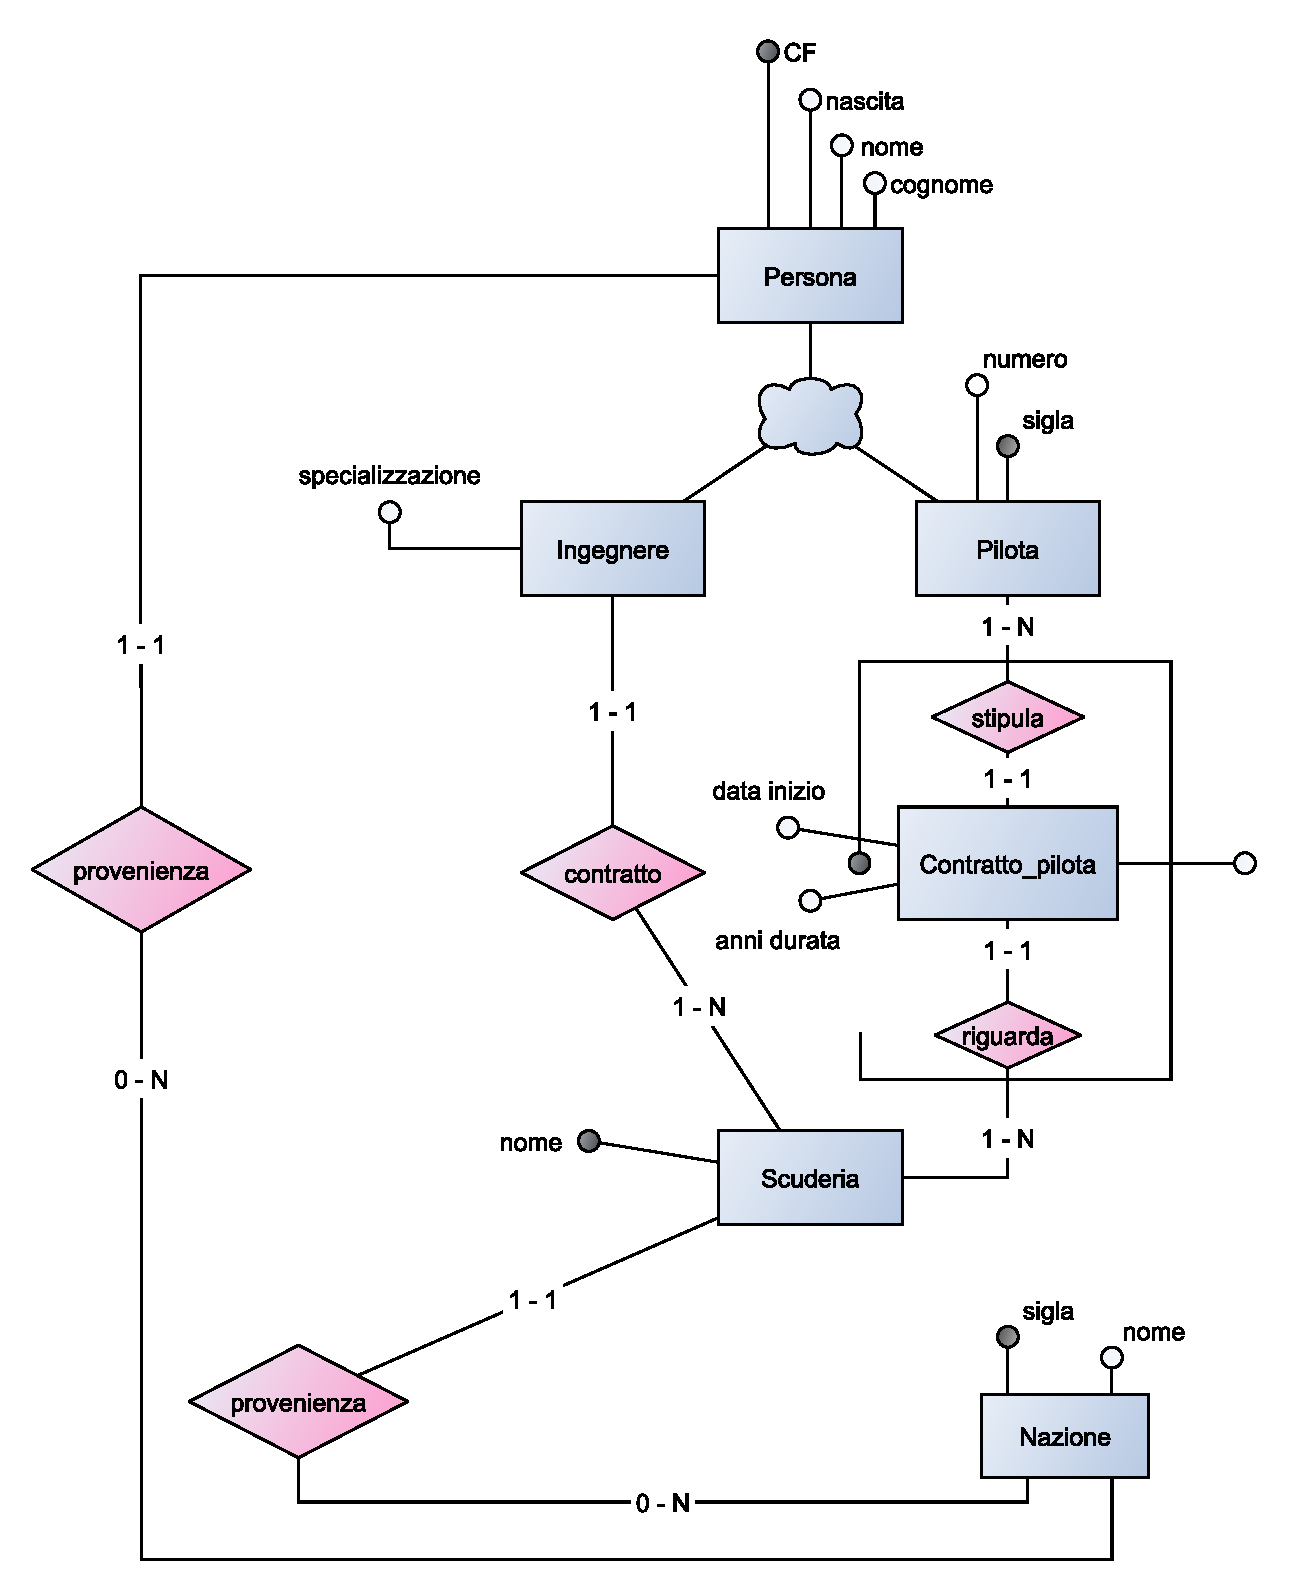
\includegraphics[scale=0.8]{copies/scheletro1.pdf}
	\end{figure}
		\section{Scuderia}
	Per ogni campionato, le scuderie schierano il veicolo derivato dalle migliorie ingegneristiche apportate al modello
	precedente. Per regolamento una scuderia può offrire ai suoi piloti solamente un modello di veicolo per campionato.
	L'unica parte dell'automobile che in molti casi non e' progettata dalla scuderia e' il motore, il quale può essere
	acquistato da un team avversario, e, a differenza delle altre componenti, non può essere modificato ad ogni campionato.
	Un campionato si svolge in più gare, ognuna delle quali prende parte in un circuito ad una certa ora e con un numero
	di giri variabile, deciso dagli organizzatori in base a diversi fattori, quali l'orario e le condizioni meteorologiche; ragione per la quale, ogni Gran Premio viene identificato dal nome del circuito e dalla data e ora del suo svolgimento, in quanto nella stessa giornata possono avvenire più gare sulla stessa pista.
	\begin{figure}[htbp]
		\centering
		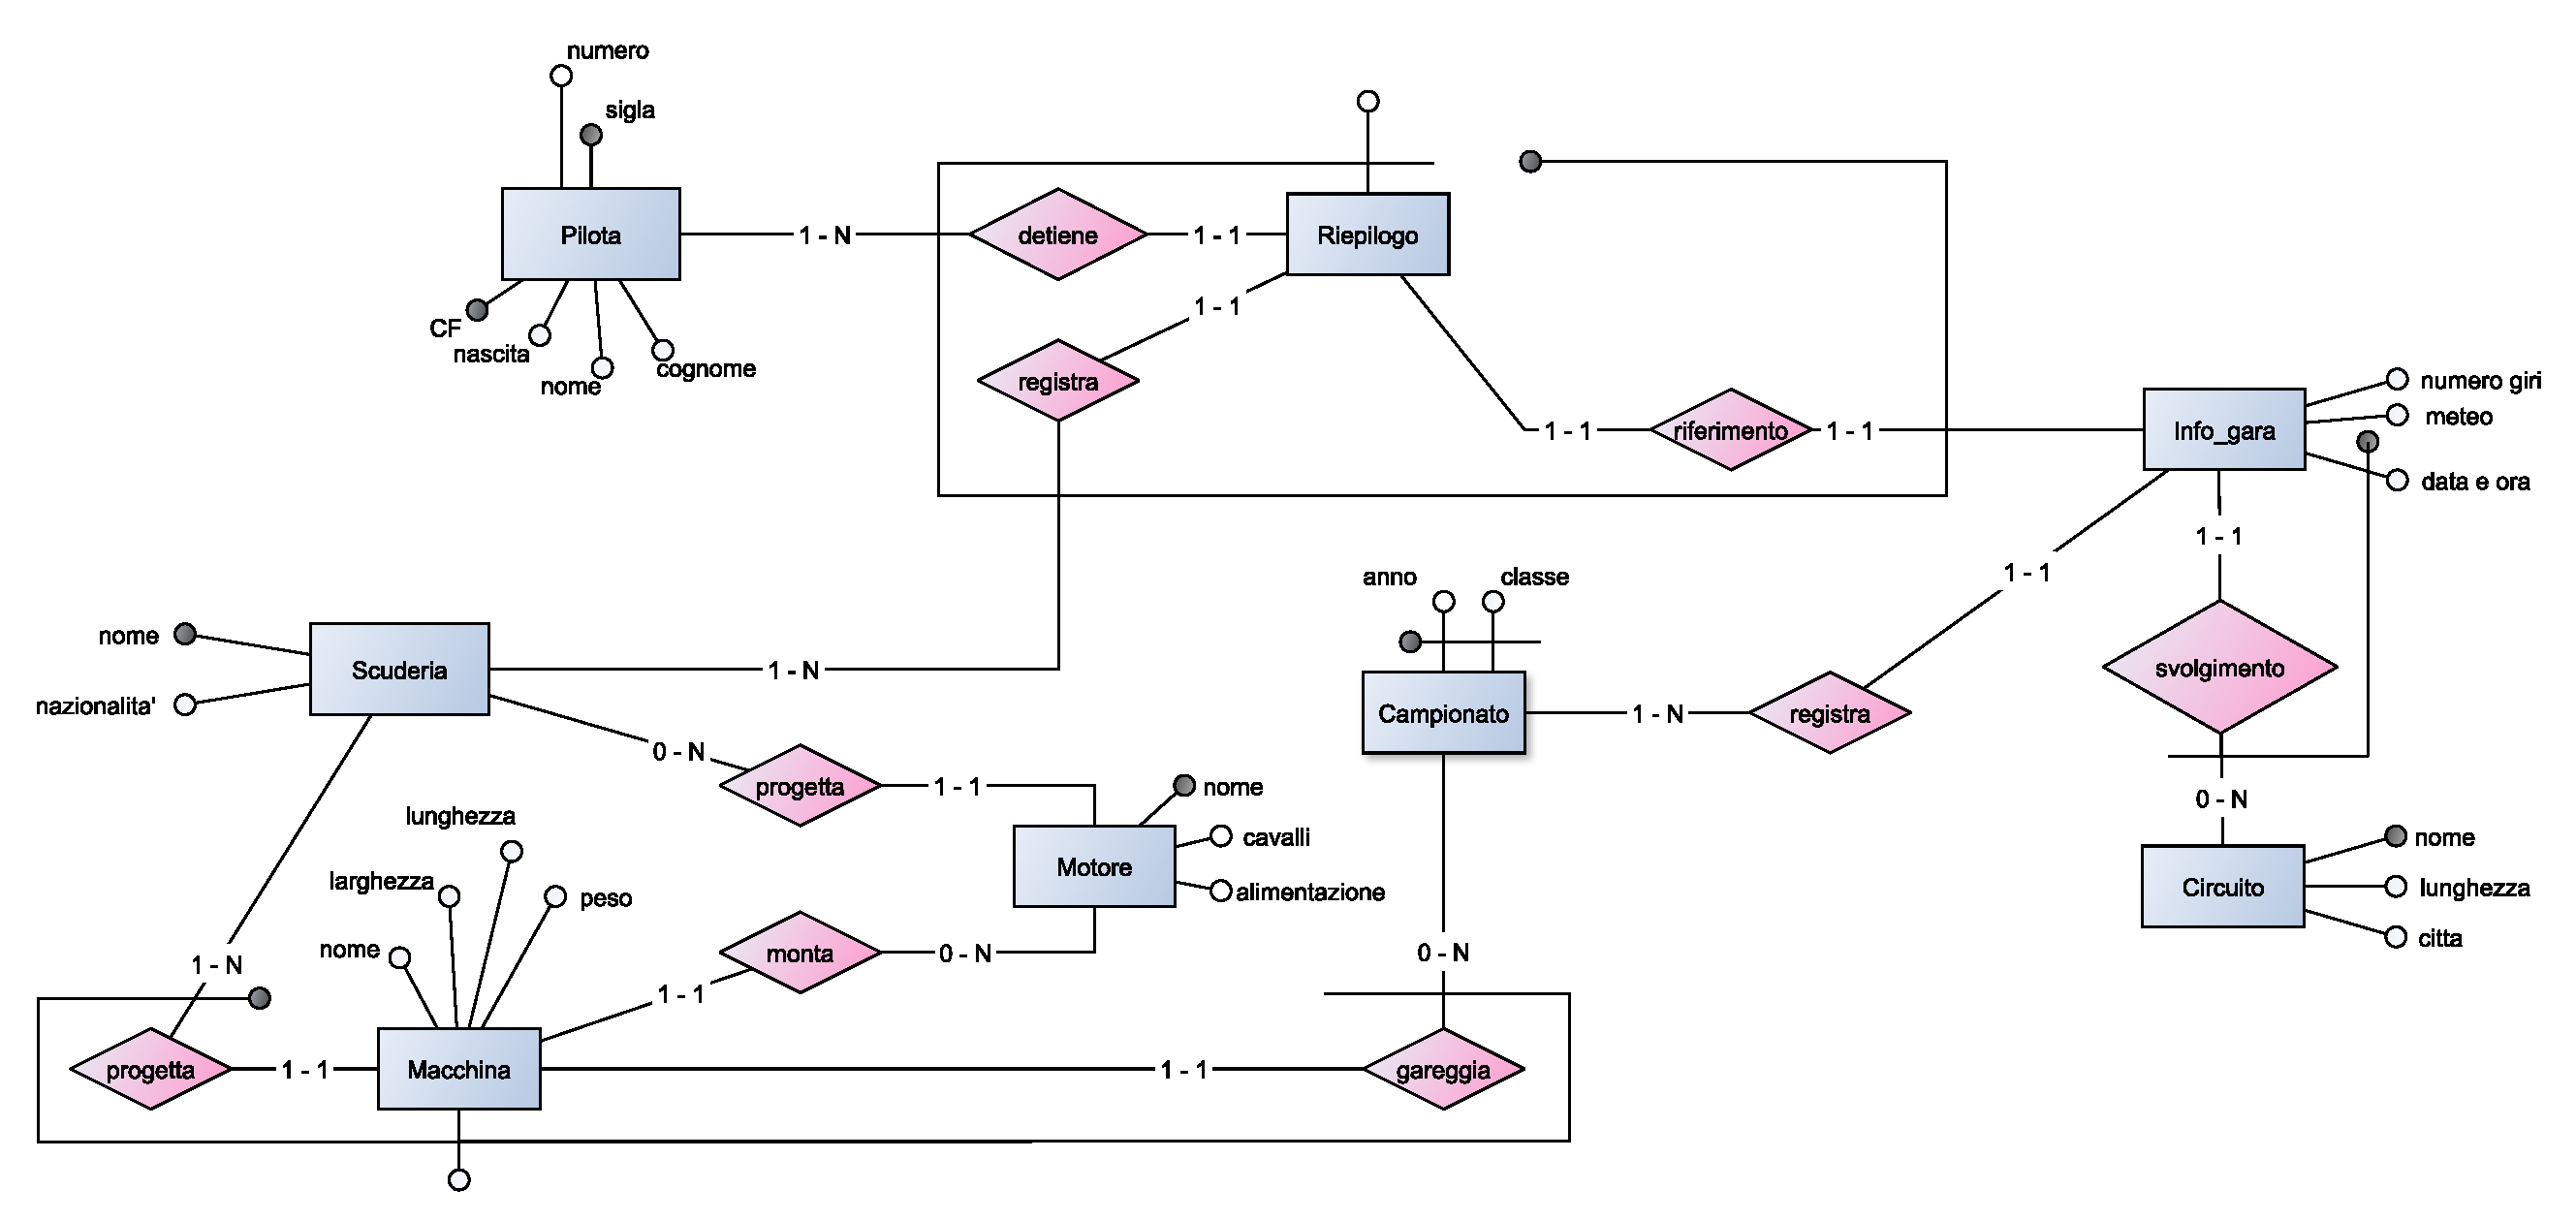
\includegraphics[scale=0.8]{copies/scheletro2.pdf}
	\end{figure}
		\section{Risultati}
	Il risultato di un pilota in una gara viene memorizzato tramite l'entità Riepilogo.
	I giri, i pit-stop ed i risultati delle gare e delle qualifiche si collegano a Riepilogo tramite chiavi esterne.
	Ogni pilota può avere solamente un Riepilogo relativo ad una gara.
	Nonostante i vincoli derivanti dal contratto tra pilota e team, in casi rari, ai corridori viene data la possibilità
	di partecipare ad una gara con una scuderia diversa da quella con la quale ha stipulato il contratto.
	\begin{figure}[htbp]
		\centering
		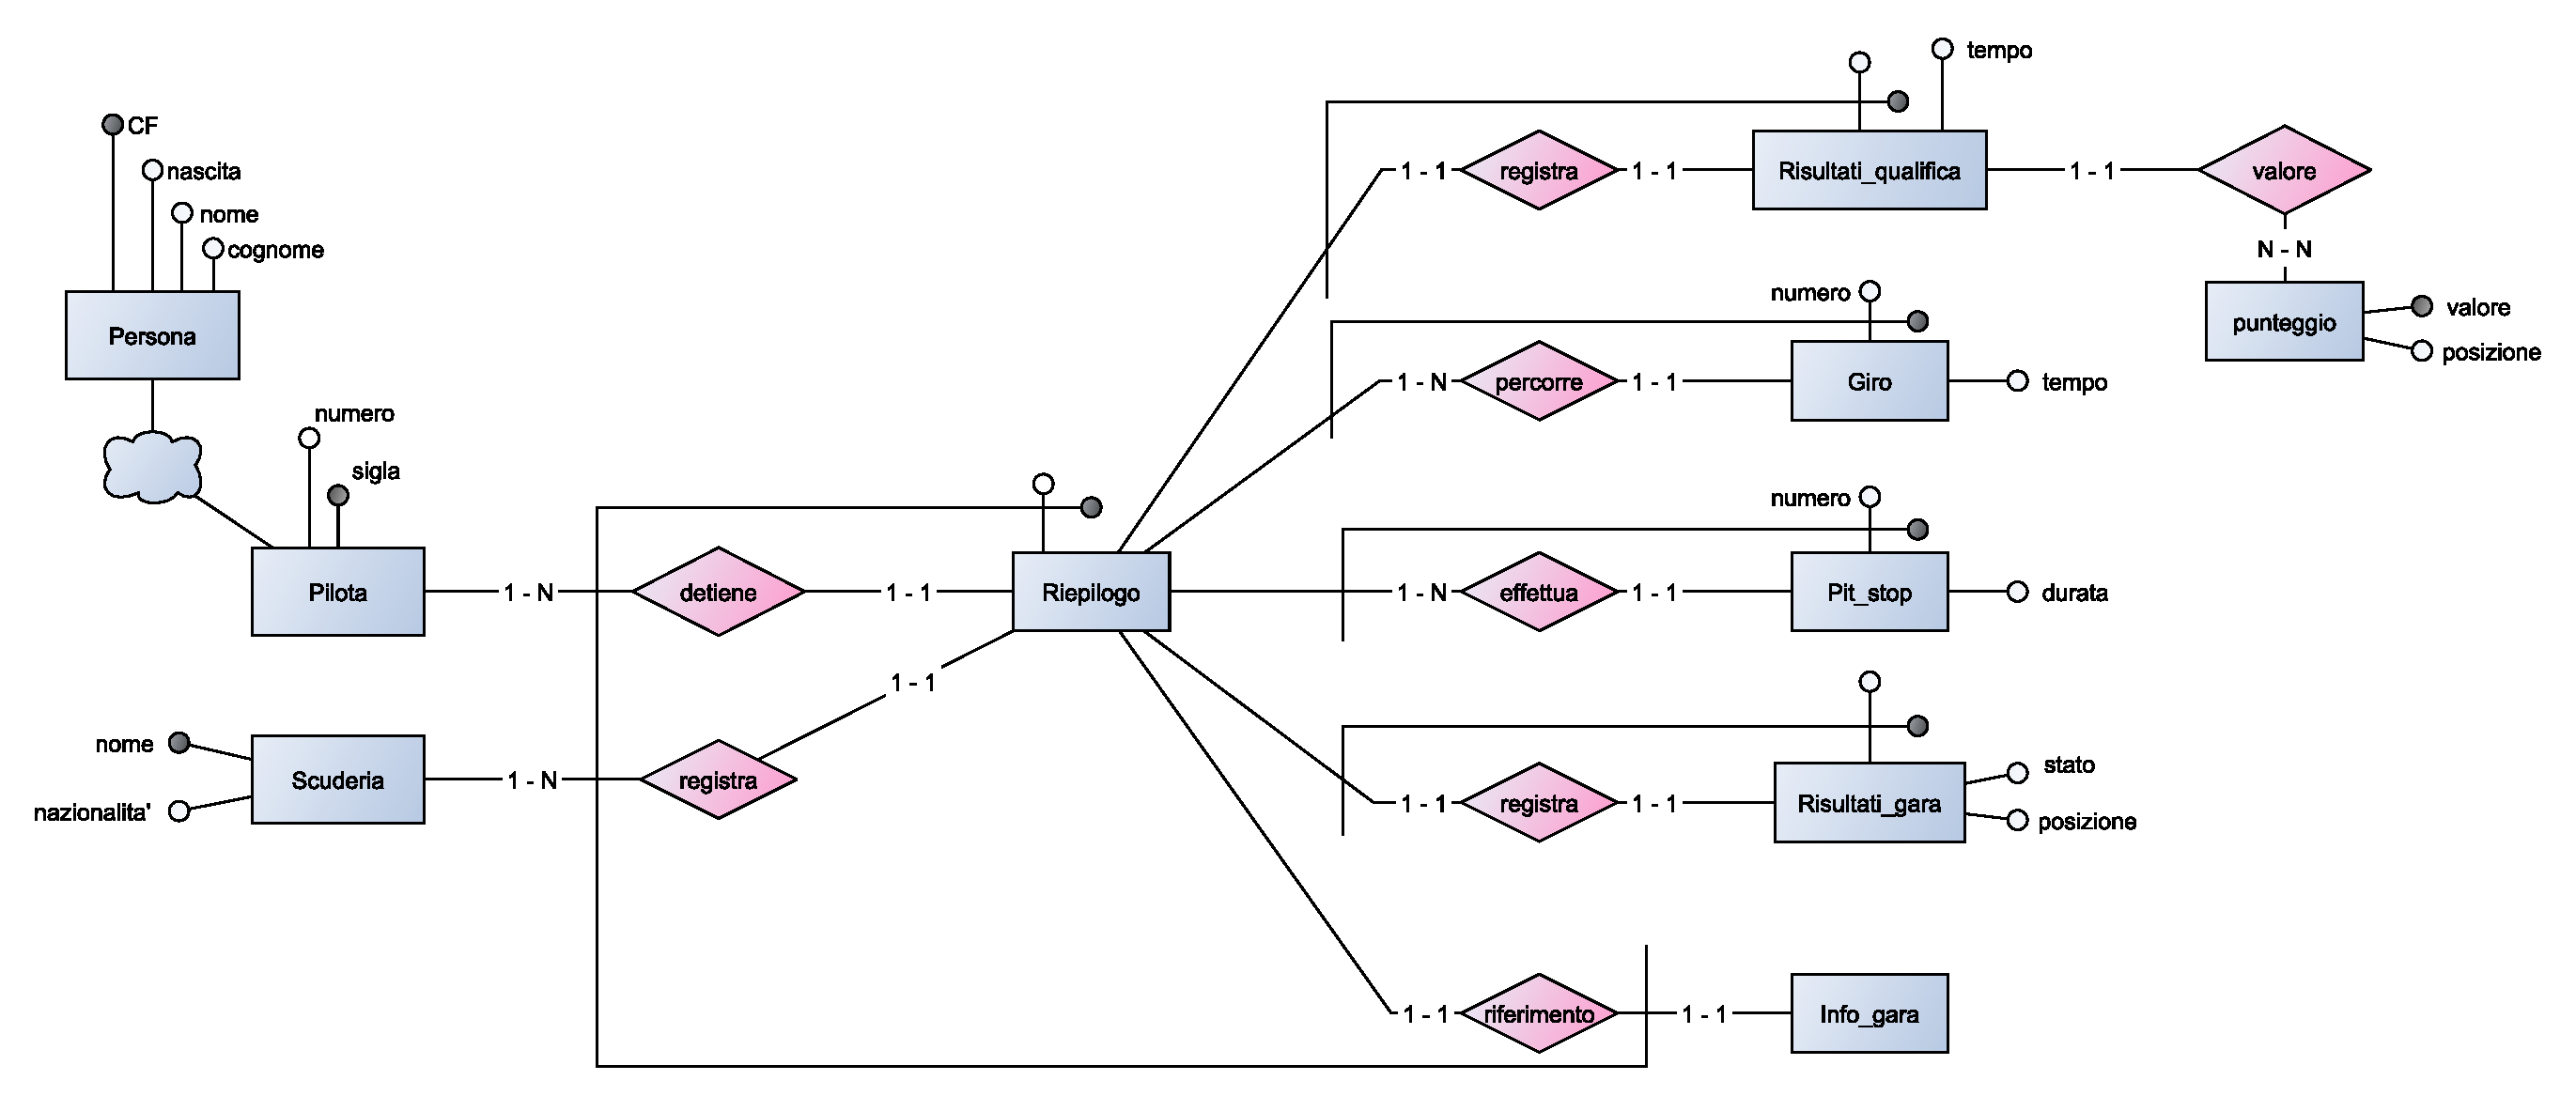
\includegraphics[scale=0.8]{copies/scheletro3.pdf}
	\end{figure}
		\section{Schema concettuale finale}
		\begin{figure}[htbp]
			\centering
			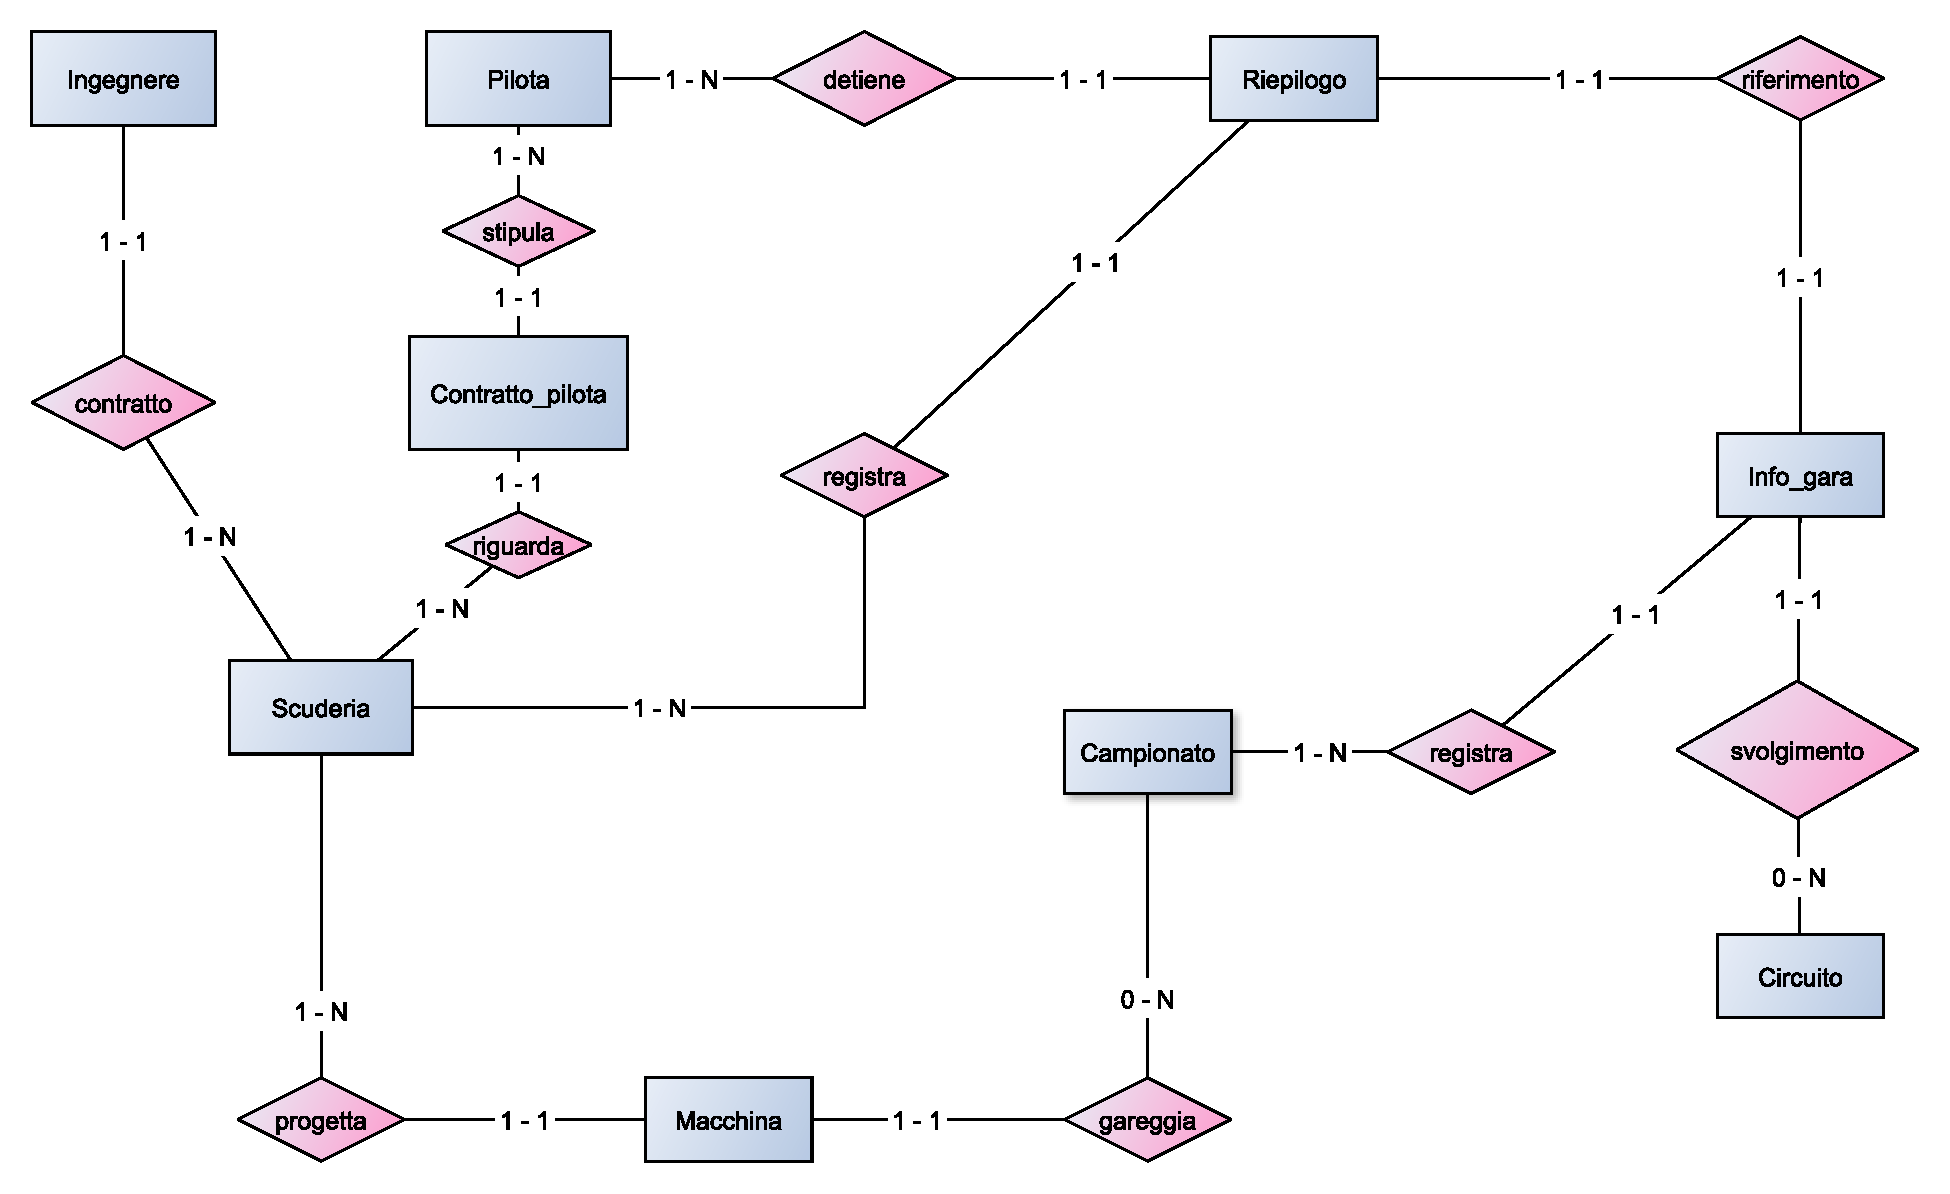
\includegraphics[scale=0.8]{copies/scheletrone.pdf}
		\end{figure}
		\section{Schema E-R finale}
		\begin{figure}[htbp]
			\centering
			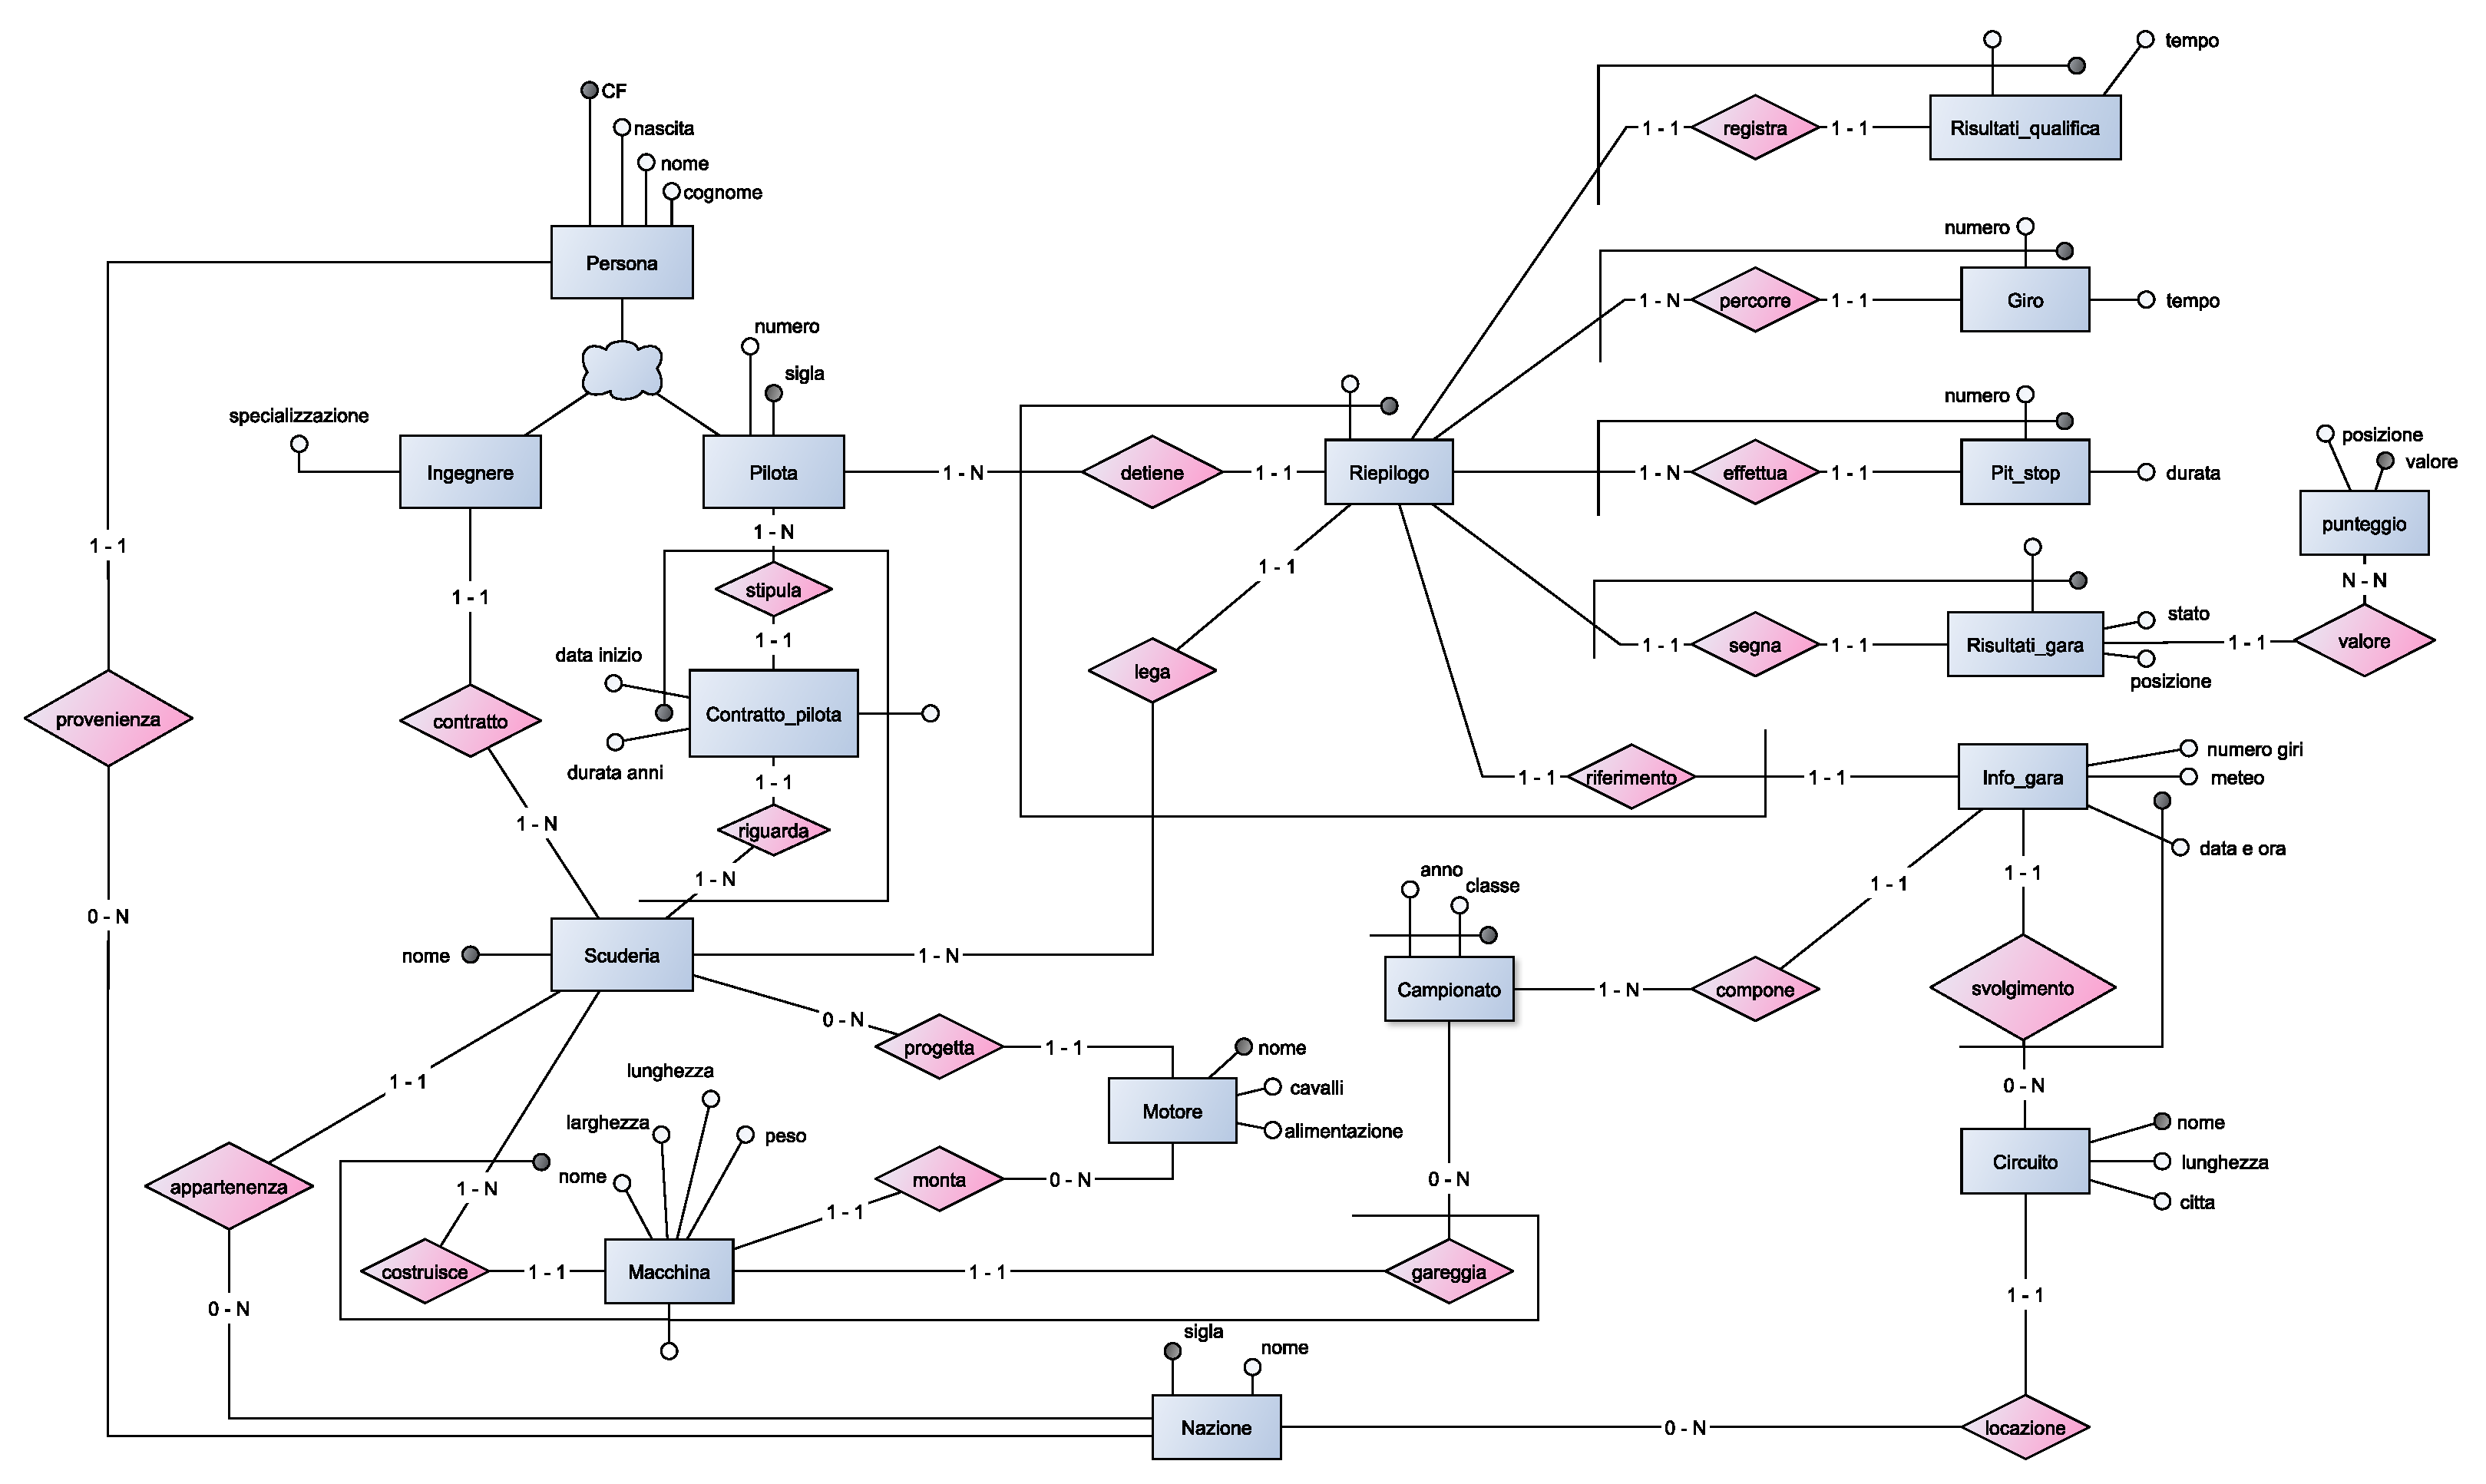
\includegraphics[scale=0.8]{copies/ERfinale.pdf}
		\end{figure}

	\chapter{Progettazione logica}
	\section{Stima volume dati}
	\hfill
	\small\addtolength{\tabcolsep}{+10pt}
	\begin{table}[h!]
		\centering
		\begin{center}
			\label{tab:table1}
			
			\scalebox{1.5}{
			\begin{tabular}{|c|c|c|} % <-- Alignments: 1st column left, 2nd middle and 3rd right, with vertical lines in between
				%\toprule
				\hline\rowcolor{green}
				\textbf{Dato} & \textbf{Tipo} & \textbf{Quantità}\\
				\hline\hline
				%\midrule		
				Nazione				&	E	&	210\\     
				Circuito			&	E 	&	100\\
				scuderia			&	E	&	40\\
				Pilota				&	E	&	110\\
				contratto\_pilota	&   R 	&	365\\
				Ingegnere			&	E 	&	2200\\
				Contratto			&	R 	&	2200\\
				Campionato			&	E	&	15\\	     
				Giro 				&	E 	&	360000\\
				info\_gara			&	E   &	300\\ 
				riepilogo			&	R	&	6000\\
				risultati\_gara		&	E	&	6000\\
				risultati\_qualifica&	E	&	6000\\
				pit\_stop			&	E	&	9000\\
				Motore				&	E	&	18\\
				Macchina			&	E	&	160\\
				Posizione			&	E	& 	20\\
				
				\bottomrule
			\end{tabular}}
		\end{center}
	\end{table}
	\section{Operazioni principali e frequenza}
	Le operazioni da effettuare sono quelle già elencate nella fase di analisi. Segue una tabella
	riportante la loro descrizione e relativa frequenza:
	
	\hfill
	\small\addtolength{\tabcolsep}{+1pt}
	\begin{table}[h!]
		\begin{center}
			\caption{Stima volume dati}
			\label{tab:table1}
			\scalebox{1.1}{
				\begin{tabular}{|l|r|} % <-- Alignments: 1st column left, 2nd middle and 3rd right, with vertical lines in between
					\toprule
					\textbf{Operazione} & \textbf{Frequenza}\\
					\midrule
					aggiungere un pilota								& 7 / anno\\
					aggiungere una scuderia								& 1 / anno\\
					aggiungere un motore								& 12 / 3 anni\\
					aggiungere macchina ad una scuderia					& 30 / anno\\
					aggiungere un circuito								& 1 / 5 anni\\
					aggiungere un campionato							& 3 / anno\\
					aggiungere gara ad un campionato					& 60 / anno\\
					aggiungere un riepilogo di un pilota				& 1200 / anno\\		
					ottenere la classifica piloti di un campionato  	& 60 / anno\\
					ottenere la classifica scuderie di un campionato 	& 60 / anno\\
					ottenere numero vittorie di ogni pilota				& 12 / anno\\
					ottenere classifica veicoli di una certa categoria	& 10 / anno\\
					\bottomrule
			\end{tabular}}
		\end{center}
	\end{table}
	\newpage
	\section{Schemi navigazione e tabelle degli accessi}
	Sono riportate in seguito le tabelle degli accessi delle operazioni sopra riportate; inoltre, ove non risulti banale, sono stati inseriti i relativi schemi di navigazione. Al fine del calcolo dei costi, si considerano di peso doppio gli accessi in scrittura rispetto a quelli in lettura.\\\\
	\subsection{aggiunta di un motore}
	Aggiunta di un motore:\\
	viene aggiunto un motore, oltre a specificarne i valori viene scelto dall'utente
	la scuderia produttrice tra le disponibili.
	\begin{table}[!htb]
		\centering
		\begin{center}
			\scalebox{1.3}{
				\begin{tabular}{|c|c|c|c|} % <-- Alignments: 1st column left, 2nd middle and 3rd right, with vertical lines in between
					\toprule
					\textbf{Concetto} & \textbf{Costrutto} & \textbf{Accessi} & \textbf{Tipo}\\
					\midrule
					scuderia 	& E & 1 & L\\
					motore	 	& E & 1 & S\\
					\bottomrule
			\end{tabular}}
			\newline\\
			1L + 1S = 36 ogni 3 anni\\
		\end{center}
	\end{table}\\
	\subsection{aggiunta di una scuderia}
	Aggiunta di una scuderia:\\
	viene aggiunta una scuderia, la nazione viene selezionata dall'utente tra quelle disponibili.
	\begin{table}[!htb]
		\centering
		\begin{center}
			\scalebox{1.3}{
				\begin{tabular}{|c|c|c|c|} % <-- Alignments: 1st column left, 2nd middle and 3rd right, with vertical lines in between
					\toprule
					\textbf{Concetto} & \textbf{Costrutto} & \textbf{Accessi} & \textbf{Tipo}\\
					\midrule
					nazione 	& E & 1 & L\\
					scuderia	& E & 1 & S\\
					\bottomrule
			\end{tabular}}
		\newline\\
		1L + 1S = 3 ogni anno\\
		\end{center}
	\end{table}\\
	\subsection{aggiunta di un pilota}
	Aggiunta di un pilota:\\
	un pilota novizio viene registrato nel database stipulando un contratto con una scuderia,
	viene letta la lista delle scuderie con la quale il pilota può eseguire il contratto.
	\begin{table}[!htb]
		\centering
		\begin{center}
			\scalebox{1.3}{
				\begin{tabular}{|c|c|c|c|} % <-- Alignments: 1st column left, 2nd middle and 3rd right, with vertical lines in between
					\toprule
					\textbf{Concetto} & \textbf{Costrutto} & \textbf{Accessi} & \textbf{Tipo}\\
					\midrule
					nazione 			& E & 1 & L\\
					scuderia			& E & 1 & L\\
					pilota 				& E & 1 & S\\
					contratto\_pilota	& R & 1 & S\\
					\bottomrule
			\end{tabular}}
		\newline\\
		2L + 2S = 42 ogni anno\\
		\end{center}
	\end{table}\\\\
	\subsection{aggiunta di una macchina ad una scuderia}
	Aggiunta di una macchina ad una scuderia:\\
	viene registrata una macchina ad una scuderia con la quale gareggiare in un certo campionato,
	vengono lette le tabelle scuderia, campionato e motore per la selezione da parte dell'utente.
	\begin{table}[!htb]
		\centering
		\begin{center}
			\scalebox{1.3}{
				\begin{tabular}{|c|c|c|c|} % <-- Alignments: 1st column left, 2nd middle and 3rd right, with vertical lines in between
					\toprule
					\textbf{Concetto} & \textbf{Costrutto} & \textbf{Accessi} & \textbf{Tipo}\\
					\midrule
					campionato 	& E & 1 & L\\
					scuderia	& E & 1 & L\\
					motore 		& E & 1 & L\\
					macchina	& E & 1 & S\\
					\bottomrule
			\end{tabular}}
		\newline\\
		3L + 1S = 150 ogni anno\\
		\end{center}
	\end{table}\\
	\newpage
	\subsection{aggiunta di un circuito}
	Aggiungere un circuito:
	viene registrato un nuovo circuito
	\begin{table}[!htb]
		\centering
		\begin{center}
			\scalebox{1.3}{
				\begin{tabular}{|c|c|c|c|} % <-- Alignments: 1st column left, 2nd middle and 3rd right, with vertical lines in between
					\toprule
					\textbf{Concetto} & \textbf{Costrutto} & \textbf{Accessi} & \textbf{Tipo}\\
					\midrule
					nazione  & E & 1 & L\\
					circuito & E & 1 & S\\
					\bottomrule
			\end{tabular}}
		\newline\\
		1L + 1S = 3 ogni 5 anni\\
		\end{center}
	\end{table}\\
	\subsection{aggiunta di un campionato}
	Aggiungere un campionato:
	viene aggiunto un nuovo campionato, specificandone l'anno e la classe di veicoli concorrenti
	\begin{table}[!htb]
		\centering
		\begin{center}
			\scalebox{1.3}{
				\begin{tabular}{|c|c|c|c|} % <-- Alignments: 1st column left, 2nd middle and 3rd right, with vertical lines in between
					\toprule
					\textbf{Concetto} & \textbf{Costrutto} & \textbf{Accessi} & \textbf{Tipo}\\
					\midrule
					campionato  & E & 1 & S\\
					\bottomrule
			\end{tabular}}
		\newline\\
		1S = 6 ogni anno\\
		\end{center}
	\end{table}\\
	\subsection{aggiungere una gara ad un campionato}
	Aggiungere una gara ad un campionato:
	viene registrata una gara in un campionato, vengono accedute le tabelle
	\begin{table}[!htb]
		\centering
		\begin{center}
			\scalebox{1.3}{
				\begin{tabular}{|c|c|c|c|} % <-- Alignments: 1st column left, 2nd middle and 3rd right, with vertical lines in between
					\toprule
					\textbf{Concetto} & \textbf{Costrutto} & \textbf{Accessi} & \textbf{Tipo}\\
					\midrule
					campionato  & E & 1 & L\\
					circuito	& E & 1 & L\\
					info\_gara	& E & 1 & S\\
					\bottomrule
			\end{tabular}}
		\newline\\
		2L + 1S = 240 ogni anno\\
		\end{center}
	\end{table}\\
	\subsection{aggiungere il riepilogo di un pilota}
	Aggiungere il riepilogo in un pilota:\\
	viene registrato di un pilota il risultato nella qualifica, la posizione e lo stato di conclusione della gara,
	i tempi dei vari giri e dei pit stop effettuati, prima di effettuare l'inserimento dei dati, vengono 
	controllate le posizioni non ancora riempite nel podio per la gara richiesta, sia per i risultati
	della gara che per quelli della qualifica. In media per gara si eseguono 60 giri e 3 pit stop
	\begin{table}[!htb]
		\centering
		\begin{center}
			\scalebox{1.3}{
				\begin{tabular}{|c|c|c|c|} % <-- Alignments: 1st column left, 2nd middle and 3rd right, with vertical lines in between
					\toprule
					\textbf{Concetto} & \textbf{Costrutto} & \textbf{Accessi} & \textbf{Tipo}\\
					\midrule
					campionato  			& E & 1 	& L\\
					info\_gara				& E & 1 	& L\\
					pilota 					& E & 1 	& L\\
					scuderia				& E & 1 	& L\\
					risultati\_gara			& E & 1 	& L\\
					risultati\_qualifica 	& E & 1 	& L\\
					riepilogo 				& R & 1 	& S\\
					riepilogo 				& R & 1 	& L\\
					risultati\_gara 		& E & 1 	& S\\
					risultati\_qualifica 	& E & 1 	& S\\
					giro 					& E & 60 	& S\\
					pit\_stop 				& E & 3 	& S\\
					\bottomrule
			\end{tabular}}
		\newline\\
		7L + 66S = 8340 ogni anno\\
		\end{center}
	\end{table}\\
	\subsection{Classifica piloti nel campionato}
	una volta selezionato dall'utente un campionato, viene visualizzata la classifica dei piloti
	tenendo conto dei punteggi delle gare vinte e degli eventuali bonus derivati da giri migliori
	\begin{table}[!htb]
		\centering
		\begin{center}
			\scalebox{1.3}{
				\begin{tabular}{|c|c|c|c|} % <-- Alignments: 1st column left, 2nd middle and 3rd right, with vertical lines in between
					\toprule
					\textbf{Concetto} & \textbf{Costrutto} & \textbf{Accessi} & \textbf{Tipo}\\
					\midrule
					campionato  			& E & 1 	& L\\
					punteggi\_posizione		& E & 1		& L\\
					riepilogo 				& R & 2 	& L\\
					info\_gara				& E & 1 	& L\\
					risultati\_gara			& E & 1 	& L\\
					giro 					& E & 1 	& L\\
					\bottomrule
			\end{tabular}}
		\newline\\
		7L = 420 ogni anno\\
		\end{center}
	\end{table}\\
	\subsection{Classifica scuderie nel campionato}
	una volta selezionato un campionato, viene visualizzata la classifica delle scuderie
	\begin{table}[!htb]
		\centering
		\begin{center}
			\scalebox{1.3}{
				\begin{tabular}{|c|c|c|c|} % <-- Alignments: 1st column left, 2nd middle and 3rd right, with vertical lines in between
					\toprule
					\textbf{Concetto} & \textbf{Costrutto} & \textbf{Accessi} & \textbf{Tipo}\\
					\midrule
					campionato  			& E & 1 	& L\\
					riepilogo 				& R & 2 	& L\\
					info\_gara				& E & 1 	& L\\
					risultati\_gara			& E & 1 	& L\\
					punteggi\_posizione		& E & 1		& L\\
					giro 					& E & 1 	& L\\
					\bottomrule
			\end{tabular}}
		\newline\\
		7L = 420 ogni anno\\
		\end{center}
	\end{table}\\
	\subsection{Numero vittorie di ogni pilota}
	viene visualizzato il numero di vittorie compiute da ogni pilota nella sua carriera
	\begin{table}[!htb]
		\centering
		\begin{center}
			\scalebox{1.3}{
				\begin{tabular}{|c|c|c|c|} % <-- Alignments: 1st column left, 2nd middle and 3rd right, with vertical lines in between
					\toprule
					\textbf{Concetto} & \textbf{Costrutto} & \textbf{Accessi} & \textbf{Tipo}\\
					\midrule
					riepilogo 				& R & 1 	& L\\
					risultati\_gara			& E & 1 	& L\\
					\bottomrule
			\end{tabular}}
		\newline\\
		2L = 24 ogni anno\\
		\end{center}
	\end{table}\\
	\subsection{Classifica veicoli in una categoria}
	selezionata la categoria dei veicoli, viene visualizzata la classifica delle macchine piu' performanti in base al numero
	di giri migliori ottenuti nelle varie competizioni
	\begin{table}[!htb]
		\centering
		\begin{center}
			\scalebox{1.3}{
				\begin{tabular}{|c|c|c|c|} % <-- Alignments: 1st column left, 2nd middle and 3rd right, with vertical lines in between
					\toprule
					\textbf{Concetto} & \textbf{Costrutto} & \textbf{Accessi} & \textbf{Tipo}\\
					\midrule
					campionato 				& E & 2 	& L\\
					giro 					& E & 1 	& L\\
					riepilogo 				& R & 1 	& L\\
					macchina 				& E & 1 	& L\\
					\bottomrule
			\end{tabular}}
		\newline\\
		5L = 50 ogni anno\\
		\end{center}
	\end{table}\\


	\section{Analisi delle ridondanze}


	È stata introdotto l'attributo ridondante `posizione` all'entità risultati\_gara al fine di evitare i passi che coinvolgono il calcolo, quali, per esempio, la somma di tutti i tempi dei vari giri per calcolare in quanto un pilota ha concluso una gara;	
	Questa ridondanza semplifica notevolmente tutte le query ove è necessario calcolare la posizione dei piloti\\
	Esempio nella operazione: Classifica del campionato\\
	lettura della posizione di un pilota in una gara.\\\\
	con ridondanza:
	\begin{table}[h!]
		\centering
		\begin{center}
			\scalebox{1.3}{
				\begin{tabular}{|c|c|c|c|} % <-- Alignments: 1st column left, 2nd middle and 3rd right, with vertical lines in between
					\toprule
					\textbf{Concetto} & \textbf{Costrutto} & \textbf{Accessi} & \textbf{Tipo}\\
					\midrule
					campionato 			& E & 1 & L\\
					punteggio\_posizione & E & 1 & L\\
					riepilogo 			& R & 2 & L\\
					info\_gara 			& E & 1 & L\\
					risultati\_gara 	& E & 1 & L\\
					giro 				& E & 1 & L\\
					\bottomrule
			\end{tabular}}
		\newline\\
		7L = 420 ogni anno\\
		\end{center}
	\end{table}\\
	senza ridondanza:
	\begin{table}[h!]
		\centering
		\begin{center}
			\scalebox{1.3}{
				\begin{tabular}{|c|c|c|c|} % <-- Alignments: 1st column left, 2nd middle and 3rd right, with vertical lines in between
					\toprule
					\textbf{Concetto} & \textbf{Costrutto} & \textbf{Accessi} & \textbf{Tipo}\\
					\midrule
					campionato 				& E & 1 	& L\\
					punteggio\_posizione 	& E & 1 & L\\
					riepilogo 				& R & 2 	& L\\
					info\_gara 				& E & 1 	& L\\
					giro 					& E & 21 	& L\\
					\bottomrule
			\end{tabular}}
		\newline\\
		26L = 1560 ogni anno\\
		\end{center}
	\end{table}
	\section{Raffinamento dello schema}
	Eliminazione delle gerarchie:\\
	Per l'eliminazione della gerarchia 'Persona' si è scelto di adottare l'approccio del collasso verso il basso,
	inserendo in Ingegnere e in Pilota gli attributi prima appartenenti al padre.
	La scelta di questo approccio deriva dalla presenza dell'associazione tra Pilota e Riepilogo, la più importante dello schema, e in quanto le interazioni con i piloti sono molto più frequenti rispetto a quelle con gli ingegneri.
	\\\\
	Scelta delle chiavi primarie:\\
	Le chiavi primarie selezionate sono rimaste quasi completamente fedeli a quelle definite nello schema ER,
	a differenza dell'identificatore di Riepilogo, sostituito da un numero intero per facilitarne il successivo utilizzo
	in chiavi esterne; per lo stesso motivo, anche per le entità info\_gara e campionato è stato scelto come identificatore
	una cifra numerica.
	All'entità pilota è stata inoltre rimossa la chiave primaria CF, in quanto non più necessaria e per rendere
	più significativi i valori della tabella riepilogo, memorizzando il pilota con la sua sigla al posto che il codice fiscale.
	\section{Traduzione delle entità e associazioni in relazioni}
	Sono state eliminate le seguenti relazioni:\\\\
	provenienza:\tab 			importando nazione.sigla in Ingegnere 
	\tab\tab\tab					e Pilota, una volta rimossa la gerarchia\\\\
	appartenenza:\tab 			importando nazione.sigla in Scuderia\\\\
	contratto:\tab 				reificando l'associazione importando CF 
	\tab\tab\tab				da ingegnere e nome da scuderia\\\\
	stipula, Riguarda:\tab 		importando pilota.sigla e scuderia.nome 
	\tab\tab\tab				in contratto\_pilota\\\\
	costruisce, gareggia:\tab 	importando campionato.ID e scuderia.nome 
	\tab\tab\tab				in macchina\\\\
	progetta:\tab 				importando scuderia.nome in motore\\\\
	monta:\tab 					importando motore.nome in macchina\\\\
	locazione:\tab 				importando nazione.sigla in circuito\\\\
	svolgimento:\tab 			importando circuito.nome in info\_gara\\\\
	compone:\tab 				importando campionato.ID in info\_gara\\\\
	detiene:\tab 				importando pilota.sigla in riepilogo\\\\
	lega:\tab					importando scuderia.nome in riepilogo\\\\
	percorre:\tab				importando riepilogo.ID in giro\\\\
	effettua:\tab				importando riepilogo.ID in pit\_stop\\\\
	segna:\tab					importando riepilogo.ID in risultati\_gara\\\\
	registra:\tab				importando riepilogo.ID in risultati\_qualifica\\\\
	valore:\tab					importando punteggio.valore in risultati\_gara\\\\
	nazione(\underline{sigla}, nome)\\
	campionato(\underline{ID}, anno, classe)\\
	circuito(\underline{nome}, lunghezza, nazione:nazione, città)\\
	scuderia(\underline{nome}, nazionalità:nazione)\\
	motore(\underline{nome}, produttore:scuderia, cavalli, alimentazione)\\
	macchina(\underline{ID\_scuderia}:scuderia, \underline{ID\_campionato}:campionato, nome, cognome,
	\tab\tab motore:motore, peso, lunghezza, larghezza)\\
	pilota(\underline{sigla}, numero, nazionalità:nazione, nascita, nome, cognome)\\
	contratto\_pilota(\underline{ID\_pilota}:pilota, \underline{ID\_scuderia}:scuderia, data\_inizio, durata\_anni)\\
	punti\_posizione(\underline{posizione}, punteggio)\\
	ingegnere(\underline{CF}, specialità, nazionalità:nazione, nascita, nome, cognome)\\
	contratto(\underline{CF}:ingegnere, \underline{ID\_scuderia}:scuderia)\\
	info\_gara(\underline{ID}, data\_gara, n\_giri, meteo, circuito:circuito, campionato:campionato)\\
	riepilogo(\underline{ID}, gara:info\_gara, pilota:pilota, scuderia:scuderia)\\
	giro(\underline{ID\_riepilogo}:riepilogo, \underline{numero}, tempo)\\
	risultati\_gara(\underline{ID\_riepilogo}:riepilogo, posizione:punti\_posizione, stato)\\
	risultati\_qualifica(\underline{ID\_riepilogo}:riepilogo, posizione, tempo)\\
	pit\_stop(\underline{numero}, \underline{ID\_riepilogo}:riepilogo, durata)\\
	\section{Schema relazionale finale}
	\begin{figure}[htbp]
		\centering
		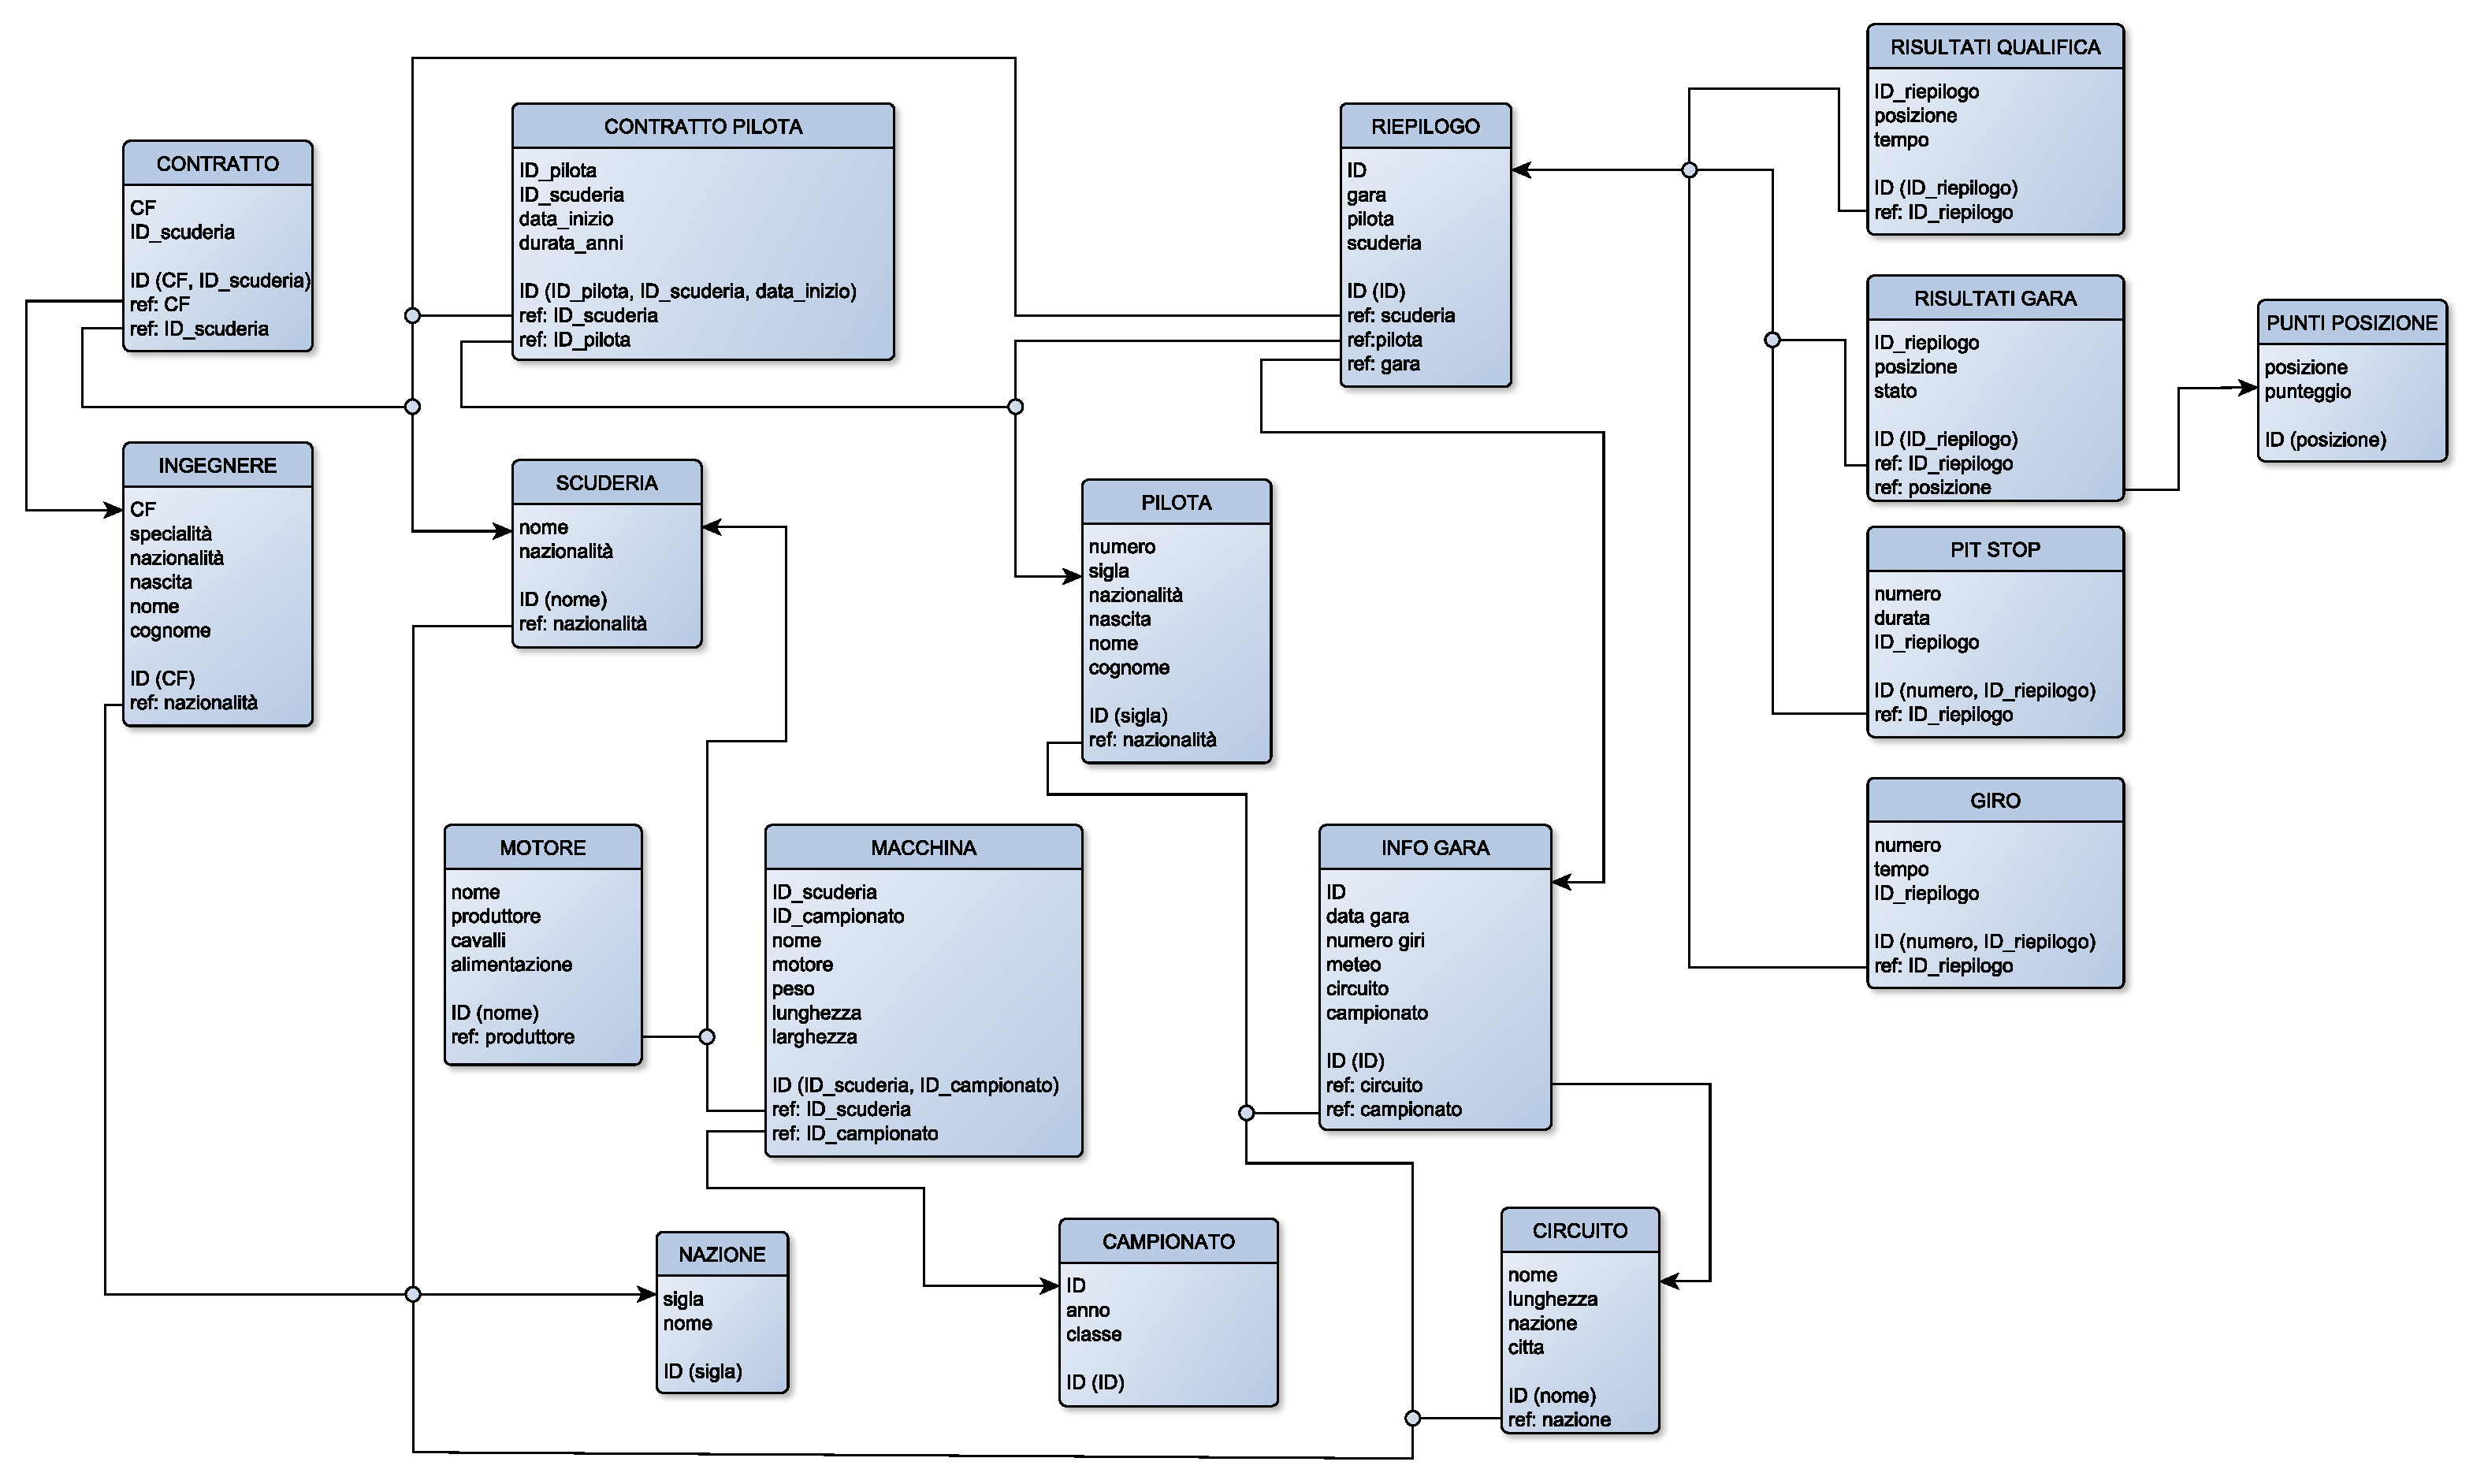
\includegraphics[scale=0.8]{copies/schemaFinale.pdf}
	\end{figure}
	\section{}
	
	\chapter{Progettazione dell'applicazione}
		\begin{table}
			\parbox{.45\linewidth}{
				\centering
				\begin{tabular}{|c|c|c|}
					\hline
					a&b&c\\
					\hline
				\end{tabular}
				\caption{Foo}
			}
			\hfill
			\parbox{.45\linewidth}{
				\centering
				\begin{tabular}{ccc}
					\hline
					d&e&f\\
					\hline
				\end{tabular}
				\caption{Bar}
			}
		\end{table}
\end{document}